\subsubsection{29.01.15 (Соревнования)}
\begin{center}
	2-ой день соревнований "Робофест-Урал"
\end{center}
Сегодня проходили квалификационные и финальные матчи.
\newline 

Внесенные доработки:
\begin{enumerate}
	\item На механизм закидывания мяча в корзину 30 см вместо проволочного крючка был установлен болт с гайками на конце, поскольку крючок гнулся после каждого закидывания и не обеспечивал гарантированного попадания мяча в корзину.
	\begin{figure}[H]
		\begin{minipage}[h]{0.2\linewidth}
			\center  
		\end{minipage}
		\begin{minipage}[h]{0.6\linewidth}
			\center{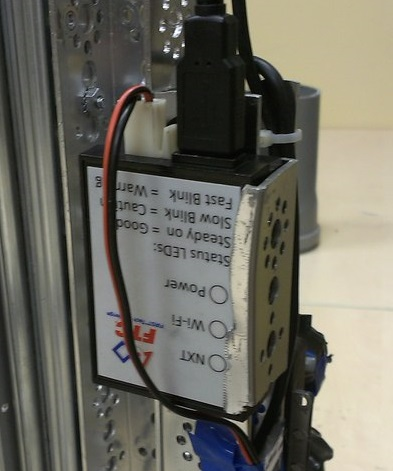
\includegraphics[scale=0.3]{days/26.01.15/images/01}}
			\caption{Доработка механизма закидывания мяча}
		\end{minipage}
	\end{figure}
	
	\item Поскольку во время проведения квалификационных матчей нашей дружественной команде, "ФМЛ№30 ${\psi}$", срочно понадобился мощный сервопривод, мы были вынуждены отдать им свой с механизма захвата корзин. В связи с этим, нам пришлось вернуть на захват корзин обычный сервопривод, что привело к возвращению старых проблем с самопроизвольным открыванием захвата в процессе движения.
	
\end{enumerate}

Результаты соревнований:
\begin{enumerate}
	\item По результатам квалификационных матчей мы заняли 3-е место.
	
	\item В финальные игры мы вышли, поскольку были выбраны командой "FTC-1", набравшей наибольшее количество побед по результатам квыалификационных матчей (по очкам мы обошли эту команду, но из-за двух поражений уступили ей первенство в квалификационных матчах).
	
	\item Наш альянс занял первое место.
	
	\item Мы также заняли 1 место в номинации "Защита инженерной книги".
	
	\item Таким образом, Мы заняли первое место в общекомандном зачете.
\end{enumerate}

Подведение итогов:
\begin{enumerate}
  \item Успешность выступления на соревнованиях:
  \begin{enumerate}
	\item По результатам игры наш альянс занял первое место.
	
	\item Мы заняли первое место в категории "Защита инженерной книги".
	
	\item В процессе игр нами не были до конца реализованы все преимущества нашего робота: автономный период из 4 квалификационных игр сработал только в последней. Также в финале в одной из игр нам удалось забросить автономный мяч в корзину 30 см, но противник, выехавший из своей зоны и перегородивший нам дорогу, помешал нам сделать все остальное. В управляемом периоде нам удалось осуществить забрасывание мячей в центральную корзину только в двух квалификационных матчах. Собирание мячей в корзину 90 см в основном периоде было осложнено тем, что во-первых мы часто наезжали на маленькие мячи, что частично (но не полностью, как на более ранних соревнованиях) ухудшало управляемость робота, а также на палку-упор, которая после рассыпания мячей продолжала лежать на поле. Кроме того, когда мы наскакивали на палку или мячи, мы теряли захваченную корзину.
	
	\item Участвуя в данном соревновании, мы выполнили главную задачу, которую мы ставили перед собой - потренироваться на официальном поле перед центральным робофестом.
	
  \end{enumerate}
  
  \item Наши ошибки и недостатки конструкции:
  \begin{enumerate}
  	\item Основной проблемой было то, что робот наезжал на мячи и палку и частично терял управление.
  	
  	\item Мы плохо подготовили автономный период и в результате смогли наладить его только к концу квалификационных матчей. Из-за этого мы не получили очков, которые могли бы заработать в автономе и не заняли 1 место по результатам квалификационных матчей.
  	
  	\item Из-за того, что ковш имел сужение в верхней части, во время опрокидывания большие мячи часто застревали поперёк него. Для того, чтобы устранить затор, нам приходилось возвращать ковш в исходное, вертикальное положение, а затем опрокидывать его снова. В результате некоторые мячи выпадали из захвата (так как ковш приходил в исходное положение резко) и мы закидывали меньшее количество мячей за один раз. Для решения этой проблемы нам будет нужно добавить в программу функцию, с помощью которой мы сможем приводить ковш в некоторое промежуточное положение, в котором мячи смогут откатываться в сторону основания ковша, освобождаясь из затора, но не смогут из него выпадать.
  	
  \end{enumerate}
  
  \item Задачи для последующих собраний:
  \begin{enumerate}
  	\item Реализовать программу автономного периода с пандуса.
  	
  	\item Подрезать лопатки захвата мячей таким образом, чтобы их длины хватало только на захват больших мячей.
  	
  	\item Реализовать защиту колес от наезда на мячи и палку-упор.
  	
  	\item Модернизировать механизм захвата корзин (МЗК) таким образом, чтобы он не терял подвижную корзину на большой скорости.
  	
  	\item Реализовать в программе управления ковшом промежуточное положение.
  	
  	\item Написать качественную речь защиты технической книги на английском и потренироваться ее рассказывать.
  	  	
  	\item Попробовать установить у себя СУИП (систему управления игровым полем) для тренировок в максимально приближенных к реальности условиях.
  	
  	\item Установить на робота защиту из листов оргстекла. Это будет не только эффективно, но и будет красиво выглядеть.
  	
  \end{enumerate}
  
\end{enumerate}
\fillpage